\documentclass[serif,mathserif]{beamer}
\usepackage{amsmath, amsfonts, epsfig, xspace}
\usepackage{algorithm,algorithmic}
\usepackage{pstricks,pst-node}
\usepackage{multimedia}
\usepackage[normal,tight,center]{subfigure}
\setlength{\subfigcapskip}{-.5em}
\usepackage{beamerthemesplit}
\usetheme{lankton-keynote}
\usepackage{CJKutf8}

\author[Group 10]{李声涛 \quad 17214643 \quad 宋日辉 \quad 17214675 \\ 黄莉 \quad 17210000 \quad 管卓群 \quad 17210000 \\ 周晓梅 \quad 17214729}

\title[PointNet\hspace{2em}\insertframenumber/\inserttotalframenumber]{PointNet: Deep Learning on Point Sets for 3D Classification and Segmentation}

\date{December 19, 2017} %leave out for today's date to be insterted

\institute{School of Data and Computer Science, SYSU}

\begin{document}
\begin{CJK*}{UTF8}{gbsn}
  \maketitle
\end{CJK*}

% \section{Introduction}  % add these to see outline in slides

\begin{frame}
  \frametitle{Content}
  \begin{itemize}
  	\item Introduction
  	\item Problem Statement
  	\item Deep Learning on Point Sets
  	\item Experiment
  	\item Conclusion
  \end{itemize}
\end{frame}

\begin{frame}{Introduction}
	\begin{itemize}
		\item Point Set
	\end{itemize}
	\begin{figure}[t]
		\centering
		\subfigure[2D Point Set]{
			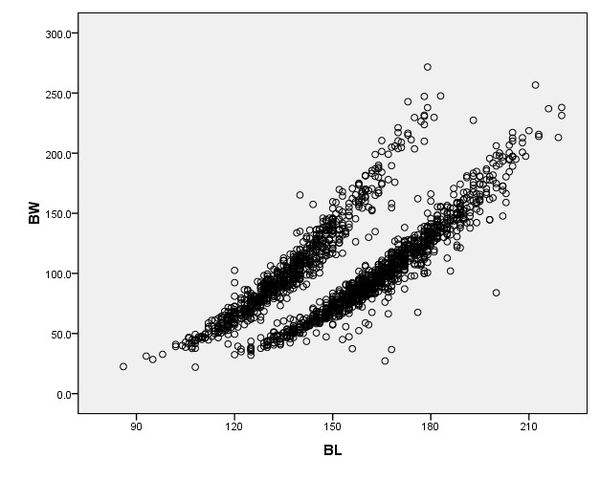
\includegraphics[width=5cm]{image/timg.jpeg}}
		\subfigure[3D Point Set (Point Cloud)]{
			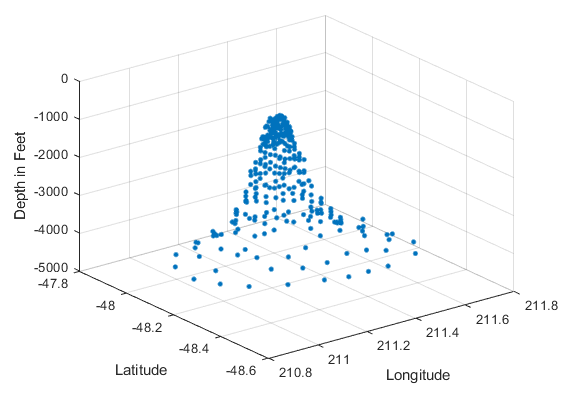
\includegraphics[width=5cm]{image/point_cloud.png}}
	\end{figure}
\end{frame}

\begin{frame}{Traditional Point Cloud Processing}
	%\begin{columns}
	%	\column{0.5\textwidth}
		\begin{itemize}
			\item Edge-based methods
			\item Model-based methods
			\item Region-based methods
			\item Attributes-based methods
			\item Graph-based methods
		\end{itemize}
	%	\column[]{0.7\textwidth}
		\begin{figure}
			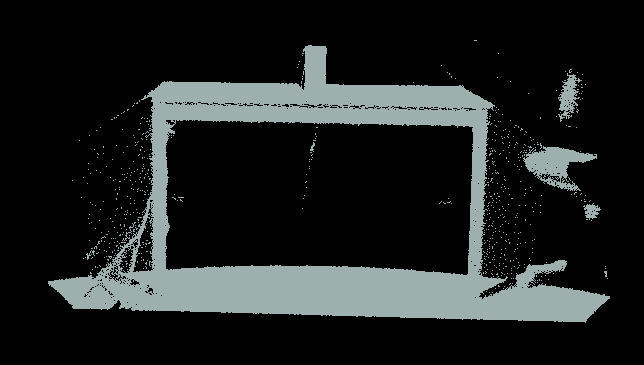
\includegraphics[width=6cm]{image/desk.png} 
			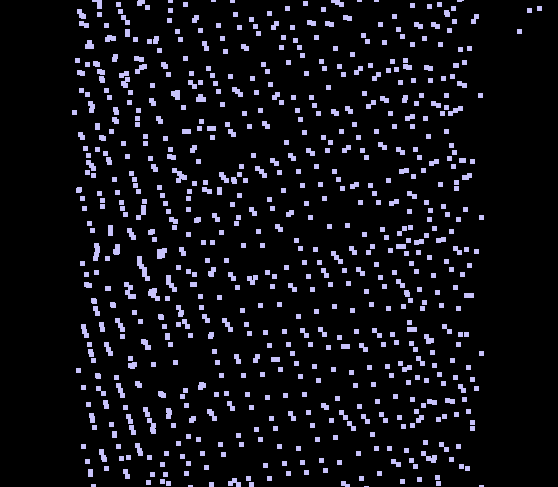
\includegraphics[width=2cm]{image/leg.png} 
		\end{figure}
%	\end{columns}
	
\end{frame}

\begin{frame}{Neural Network Based Methods}
	\begin{itemize}
		\item Volumetric CNNs: 3D voxel grids
		\begin{itemize}
			\item Constrained by resolution
		\end{itemize}
		\item Multi-view CNNs: collections of images
		\begin{itemize}
			\item Nontrivial to extend them to scene understanding or other 3D tasks.
		\end{itemize}
	\end{itemize}
\end{frame}

\begin{frame}{PointNet}
	\begin{itemize}
		\item A novel deep net architecture
		\item Input: point set
		\item Tasks: 3D shape classification, shape part segmentation, and scene semantic parsing 
		\item Simple, effective and robust
	\end{itemize}
	\begin{figure}
		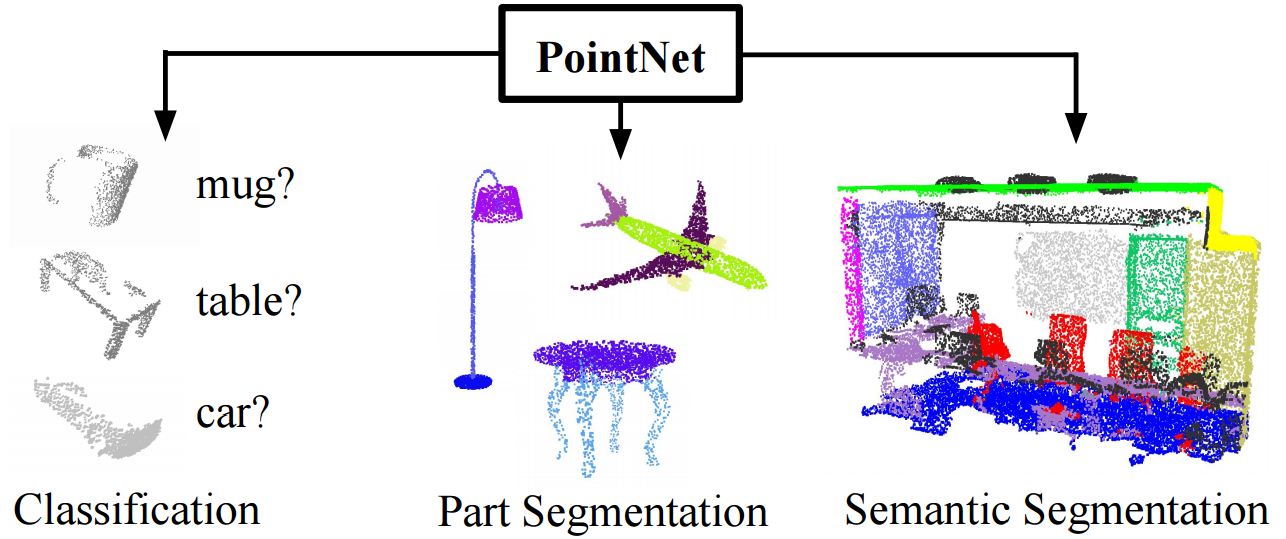
\includegraphics[width=9cm]{image/teaser.png}
	\end{figure}
\end{frame}

\begin{frame}{Problem Statement}
	...
\end{frame}

\begin{frame}{Deep Learning on Point Sets}
	...
\end{frame}

\begin{frame}{Experiments}
	...
\end{frame}

\begin{frame}{Conclusion}
	...
\end{frame}
\end{document}

%These are examples.
% \section{Main Body} % add these to see outline in slides
%
%\begin{frame}
%	\frametitle{Equations}
%	Equations are easy
%	\begin{itemize}
%		\item Just and paste equations\pause
%		\item From the paper!
%		\begin{equation*}
%		\textbf{p}^* = \underset{\textbf{p}}{\arg\!\min}~\sum_{\textbf{x}}\left[ I(\textbf{W}(\textbf{x};\textbf{p})) - T(\textbf{x}) \right]^2
%		\end{equation*}
%	\end{itemize}
%\end{frame}


%\begin{frame}
%	\frametitle{Pictures}
%	\begin{figure}[t]
%		\centering
%		\subfigure[First Frame]{
%			%    \includegraphics[width=3cm]{figures/naked_leaves/00000001}}
%			
\includegraphics[width=3cm]{image/lion.png}}
%		\subfigure[Middle Frame]{
%			%    \includegraphics[width=3cm]{figures/naked_leaves/00000120}}
%			
\includegraphics[width=3cm]{image/lion.png}}
%		\subfigure[Last Frame]{
%			%    \includegraphics[width=3cm]{figures/naked_leaves/00000240}}
%			
\includegraphics[width=3cm]{image/lion.png}}
%	\end{figure}
%\end{frame}
%
%\begin{frame}
%	\frametitle{A Movie}
%	\begin{center}
%		\movie[height=5cm,width=6.5cm,poster,autostart,loop]{}{leaves.avi}
%	\end{center}
%	\begin{itemize}
%		\item Movies only seem to work in Adobe Reader
%		\item Movie file is not embedded, it must be on the computer
%	\end{itemize}
%\end{frame}
%
%% \section{Conclusion} % add these to see outline in slides
%
%\begin{frame}
%	\frametitle{Credits}
%	\begin{itemize}
%		\item Brought to you by www.shawnlankton.com
%		\item Please let me know about improvements!
%		\item This was supposed to look like a KeyNote Show
%		\item inspiration: http://www.ucl.ac.uk/~ucbpeal/latexposter.html
%		\item inspiration: http://newsgroups.derkeiler.com/... (in code)
%		%http://newsgroups.derkeiler.com/Archive/Comp/comp.text.tex/2007-11/msg00299.html
%	\end{itemize}
%\end{frame}
%
%\begin{frame}
%	\frametitle{Questions}
%\end{frame}